\documentclass{article}

\usepackage{amsmath, mathtools, amsthm, booktabs, float, hyperref}

\usepackage{graphicx}
\graphicspath{ {../images/tps/} }

\title{Centralina di irrigazione}
\author{Lena Giovanni Leonardo 5AL}
\date{Lunedì 18 Ottobre 2021}

\begin{document}
    \maketitle

    \section{Criteri}

    \begin{enumerate}
        \item Ci deve essere un controllo di accensione generale, (INGRESSO ON/OFF)
        \item La pompa può essere azionata solo se il livello del serbatoio è superiore ad una soglia indicata da un sensore di livello (INGRESSO LIVELLO)
        \item L’irrigazione può essere effettuata solo se siamo di notte, possiamo usare una fotocellula oppure un timer (INGRESSO ABILITAZIONE)
        \item ovviamente si irrigherà soltanto se un sensore di umidità posto nel terreno indicherà se il terreno è asciutto e non umido (INGRESSO UMIDITA’)
        \item Si deve prevedere anche un ingresso che viene attivato se la pompa si trova in avaria (INGRESSO PROTEZIONE), con eventuale accensione di un’uscita (USCITA AVARIA).
        \item Si deve prevedere un'uscita che segnala il livello dell'acqua troppo basso per poter eseguire l'irrigazione.
    \end{enumerate}

    \section{Lista ingressi}

    \begin{enumerate}
        \item Generale (attivo alto, interruttore generale, senza il sistema non funziona)
        \item Livello OK (attivo alto, sensore che indica il livello dell'acqua)
        \item Abilitazione notte (attivo alto, sensore che indica se l'orario è notturno)
        \item Umidità OK (attivo alto, sensore che indica se il livello dell'umidità va bene per l'irrigazione)
        \item Protezione OK (attivo basso, sensore che rileva se la pompa non si trova in avaria)
    \end{enumerate}

    \section{Lista uscite}

    \begin{enumerate}
        \item Pompa (attivo alto, aziona la pompa)
        \item Avaria (attivo alto, aziona un'indicatore che annuncia lo stato di avaria)
        \item No acqua (attivo alto, aziona un'indicatore che annuncia lo stato di mancanza dell'acqua)
    \end{enumerate}

    \section{Diagramma a stati}

    \begin{center}
        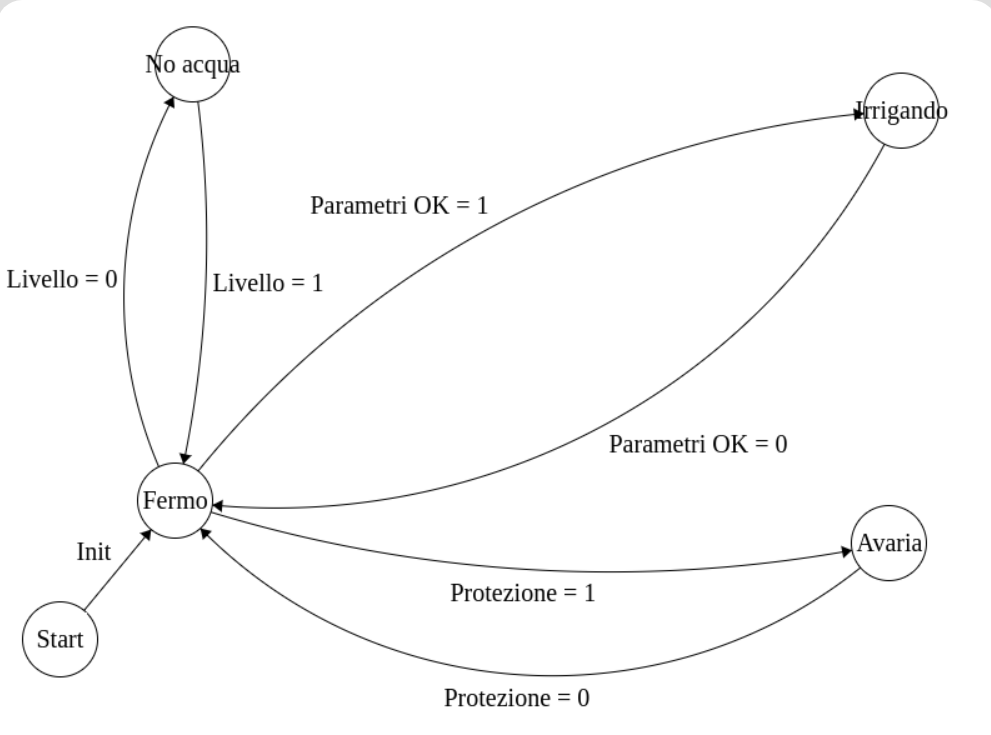
\includegraphics[width=\textwidth]{irrigazione_stati.png}
    \end{center}

    \section{Layout impianto}

    \begin{center}
        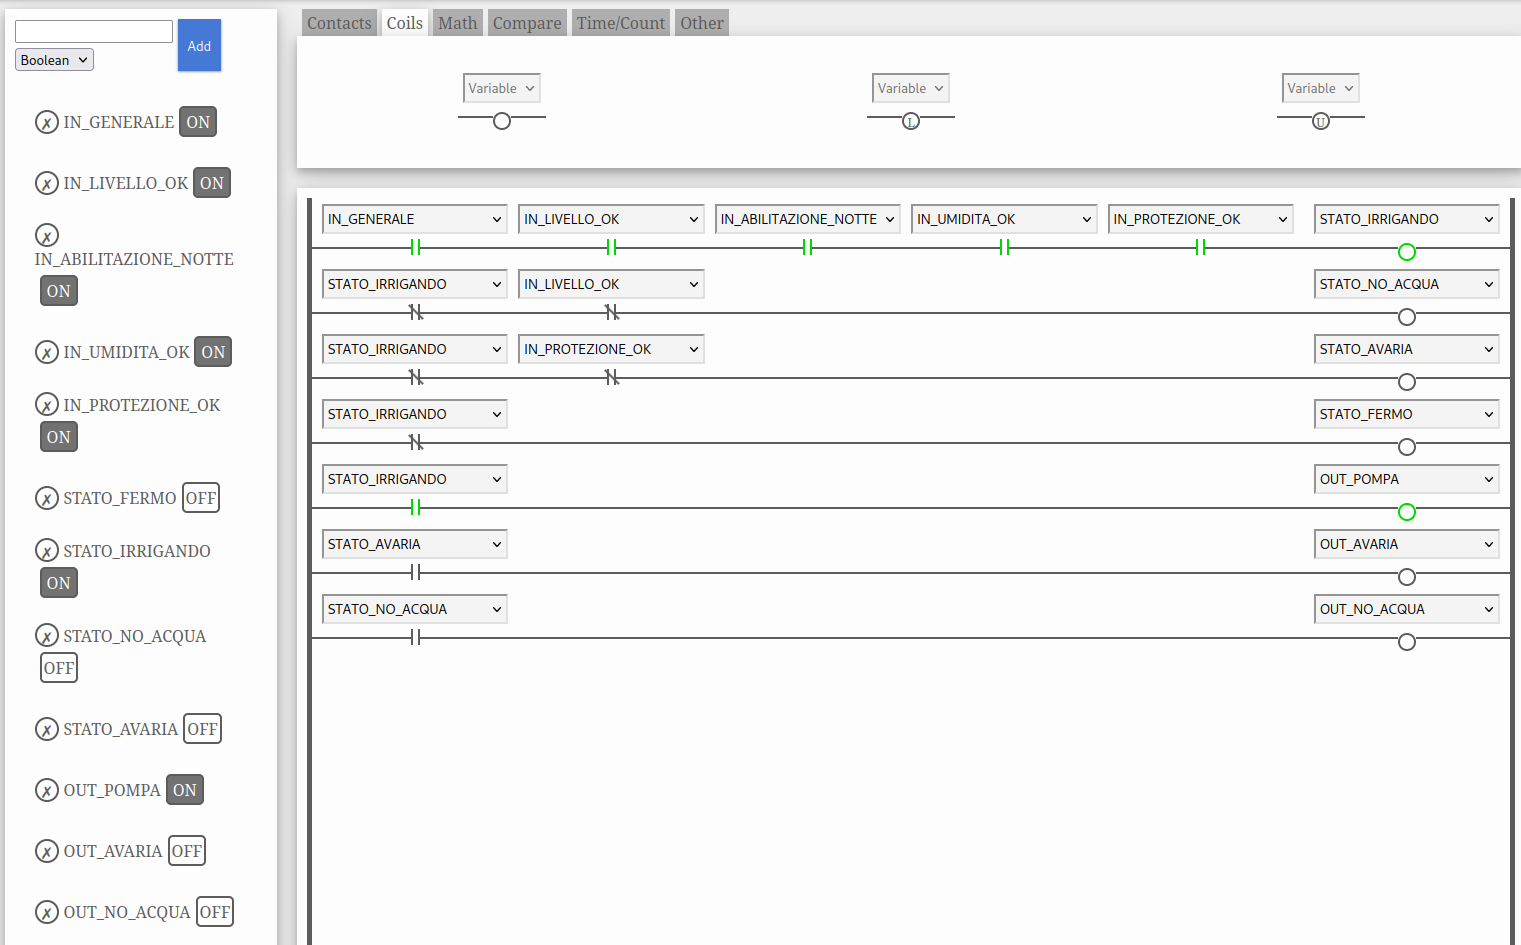
\includegraphics[width=\textwidth]{esercizio_irrigazione.png}
    \end{center}

    Dato che il simulatore di PLC utilizzato non dispone di un SuperMerker, l'implementazione inizia direttamente nello STATO\_FERMO. Nel caso in cui tutti e cinque gli ingressi necessari all'azionamento del sistema siano attivi e vibili nella prima riga dell'impianto, lo stato del sistema passa a STATO\_IRRIGANDO. In questo momento, l'unico modo per tornare indietro da questo stato è se almeno uno degli input diventi basso. In questo caso, una volta che lo stato è stato cambiato, ci sono tre possibilità:

    \begin{enumerate}
        \item lo stato rimane su STATO\_FERMO perchè non ci sono problemi da segnalare
        \item lo stato passa a STATO\_AVARIA perchè è stata rilevata un'avaria sul motore
        \item lo stato passa a STATO\_NO\_ACQUA perchè il sensore del serbatoio ha rilevato un livello troppo basso di acqua.
    \end{enumerate}

    \section{Tabella di verità (solo uscita pompa)}

    \begin{table}[H]
    \centering
    \resizebox{\textwidth}{!}{
    \begin{tabular}{|l|l|l|l|l|l|}
    \hline
    Generale & Livello & Abilitazione & Umidità & Protezione & Pompa \\ \hline
    1        & 1       & 1            & 1       & 1          & 1     \\ \hline
    0        & *       & *            & *       & *          & 0     \\ \hline
    *        & 0       & *            & *       & *          & 0     \\ \hline
    *        & *       & 0            & *       & *          & 0     \\ \hline
    *        & *       & *            & 0       & *          & 0     \\ \hline
    *        & *       & *            & *       & 0          & 0     \\ \hline
    \end{tabular}
    }
    \end{table}

    (* indica qualsiasi valore)

    \section{Tabella di verità (solo uscita avaria)}

    \begin{table}[H]
    \centering
    \resizebox{\textwidth}{!}{
    \begin{tabular}{|l|l|l|l|l|l|}
    \hline
    Generale & Livello & Abilitazione & Umidità & Protezione & Avaria \\ \hline
    *        & *       & *            & *       & 1          & 0      \\ \hline
    *        & *       & *            & *       & 0          & 1      \\ \hline
    \end{tabular}
    }
    \end{table}

    (* indica qualsiasi valore)

    \section{Tabella di verità (solo uscita no acqua)}

    \begin{table}[H]
    \centering
    \resizebox{\textwidth}{!}{
    \begin{tabular}{|l|l|l|l|l|l|}
    \hline
    Generale & Livello & Abilitazione & Umidità & Protezione & No acqua \\ \hline
    *        & 0       & *            & *       & *          & 1      \\ \hline
    *        & 1       & *            & *       & *          & 0      \\ \hline
    \end{tabular}
    }
    \end{table}

    (* indica qualsiasi valore)

    \section{Versione interattiva Ladder}

    \href{https://www.plcfiddle.com/fiddles/0ba557fc-5503-49ed-a362-f94b0fa231a3}{https://www.plcfiddle.com/fiddles/0ba557fc-5503-49ed-a362-f94b0fa231a3}

\end{document}
